%%%%%%%%%%%%%%%%%%%%%%%%%%%%%%%%%------- FIGURES -------%%%%%%%%%%%%%%%%%%%%%%%%%%%%%%%%%%

\newpage

%%%%%% FIGURE 1 %%%%%%%
\begin{figure}[h]
\centering
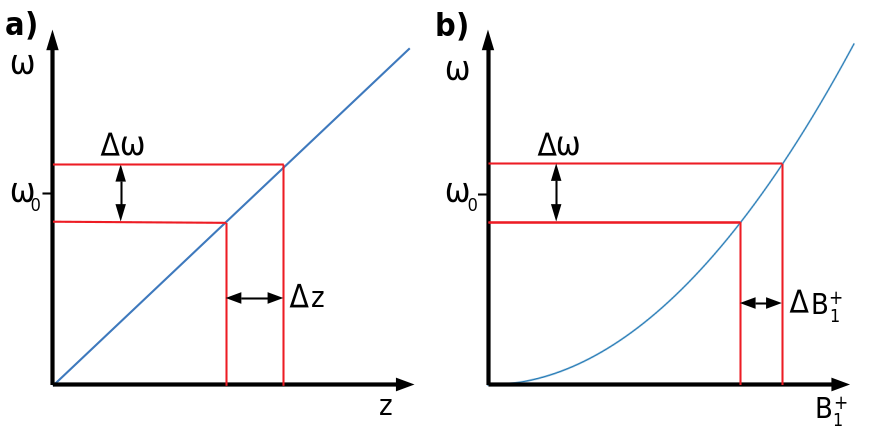
\includegraphics[width=0.75\textwidth]{figures/intro_figure.png}
\caption{a) Conventional slice selection, in which a linear gradient in the $B_0$ field introduces a spatial variation in resonant frequencies. 
When paired with a frequency-selective excitation pulse with center frequency $\omega_0$ and bandwidth $\Delta z$ a spatial slice of thickness $\Delta z$ is excited. 
b) Bloch-Siegert shift-localized slice selection, 
in which an off-resonant RF pulse produces an approximately quadratic variation in resonant frequencies across field strengths $B_1^+$. 
When paired with a frequency-selective excitation pulse, this results in the excitation of spins across a range $\Delta B_1^+$, which can be mapped to space using an amplitude gradient transmit coil.}
\label{fig:intro}
\end{figure}

%%%%%% FIGURE 2 %%%%%%%
\begin{figure}[h]
\centering
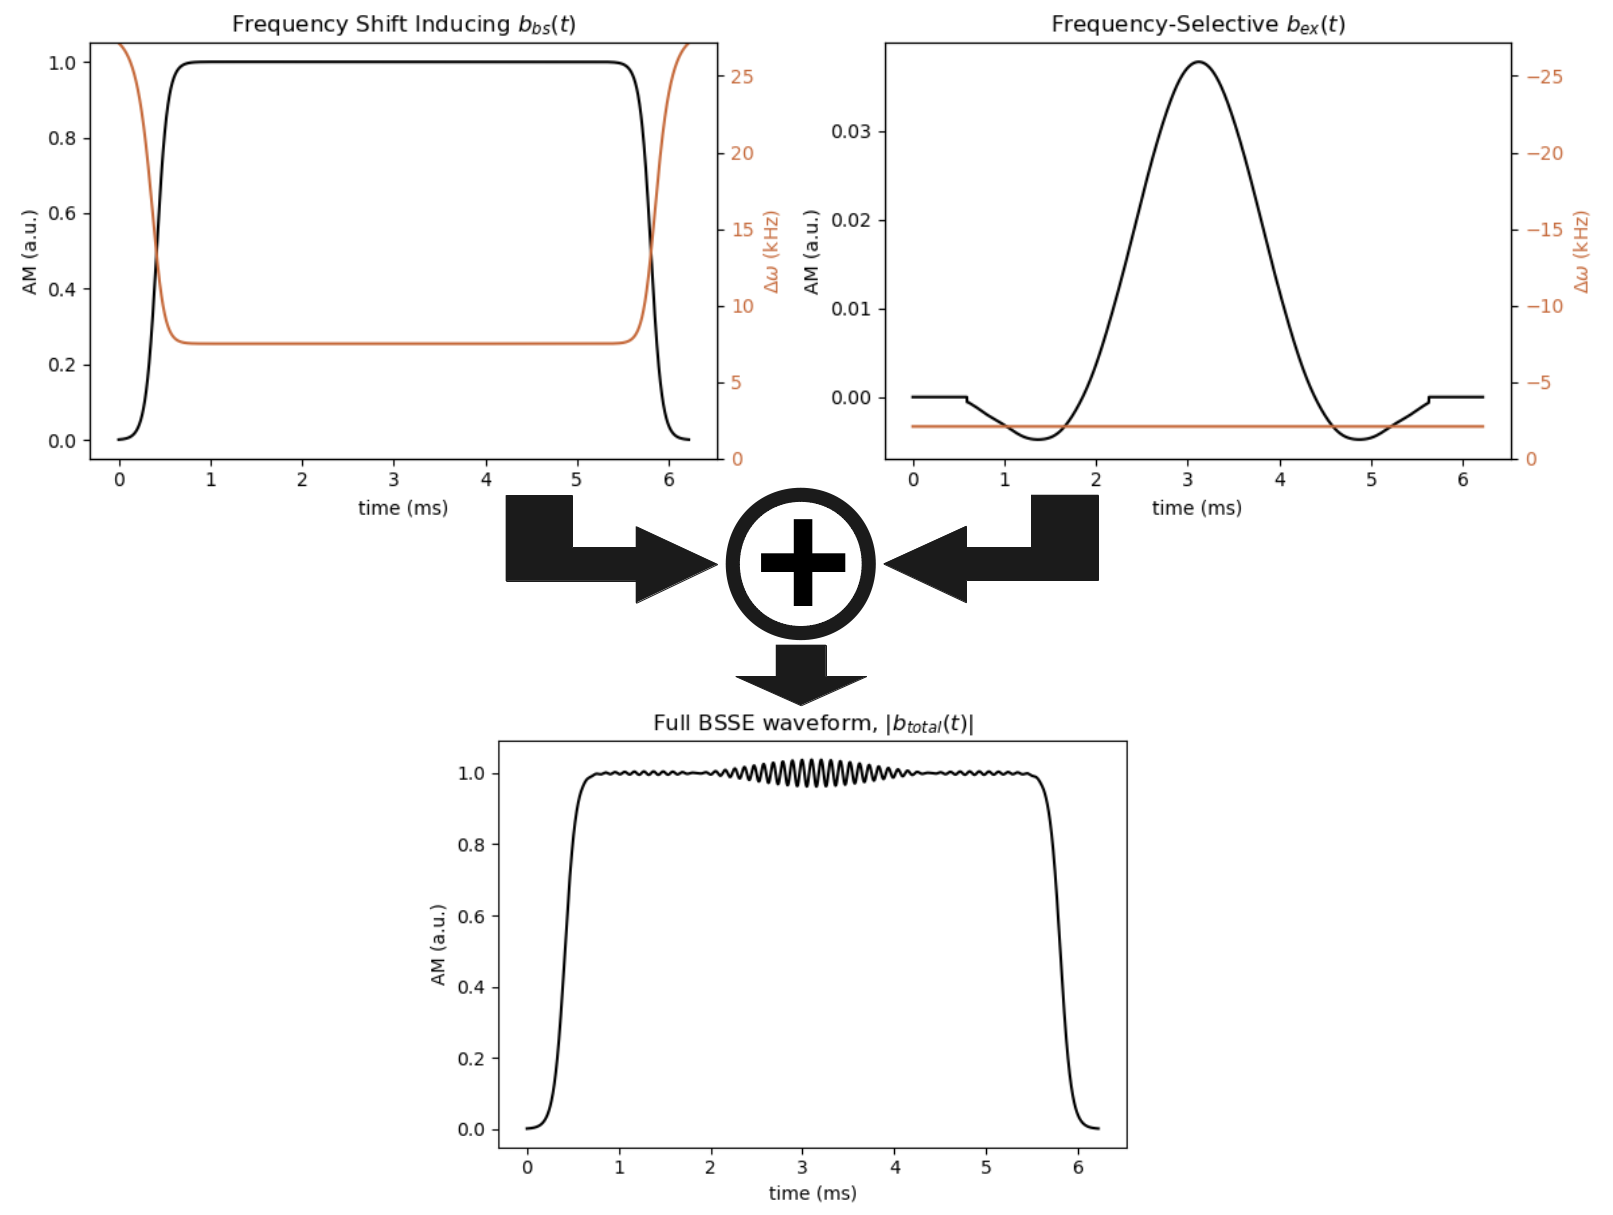
\includegraphics[width=1.1\textwidth]{figures/pulse_construction.png}
\caption{Construction of the full $b_{total}(t)$ BSSE RF pulse. The Bloch-siegert shift producing pulse $b_{bs}(t)$ (top left) and slice-selective pulse $b_{ex}(t)$ (top right) are designed independently and summed into the full BSSE waveform $b_{total}(t)$ (bottom). $b_{bs}(t)$ has Fermi AM (black) and adiabatic frequency sweeps towards and away from a constant frequency offset $\omega_{off}$ (orange). $b_{ex}(t)$ has SLR-designed AM (black) and a constant frequency offset (orange). 
Note that the amplitude of the BS waveform is generally much larger than that of the SS waveform; in $|b_{total}(t)|$, $b_{ex}(t)$ is visible as a small ripple present in the plateau of the Fermi waveform.}
\label{fig:alg}
\end{figure}

%%%%%% FIGURE 3 %%%%%%%
\begin{figure}[h]
\centering
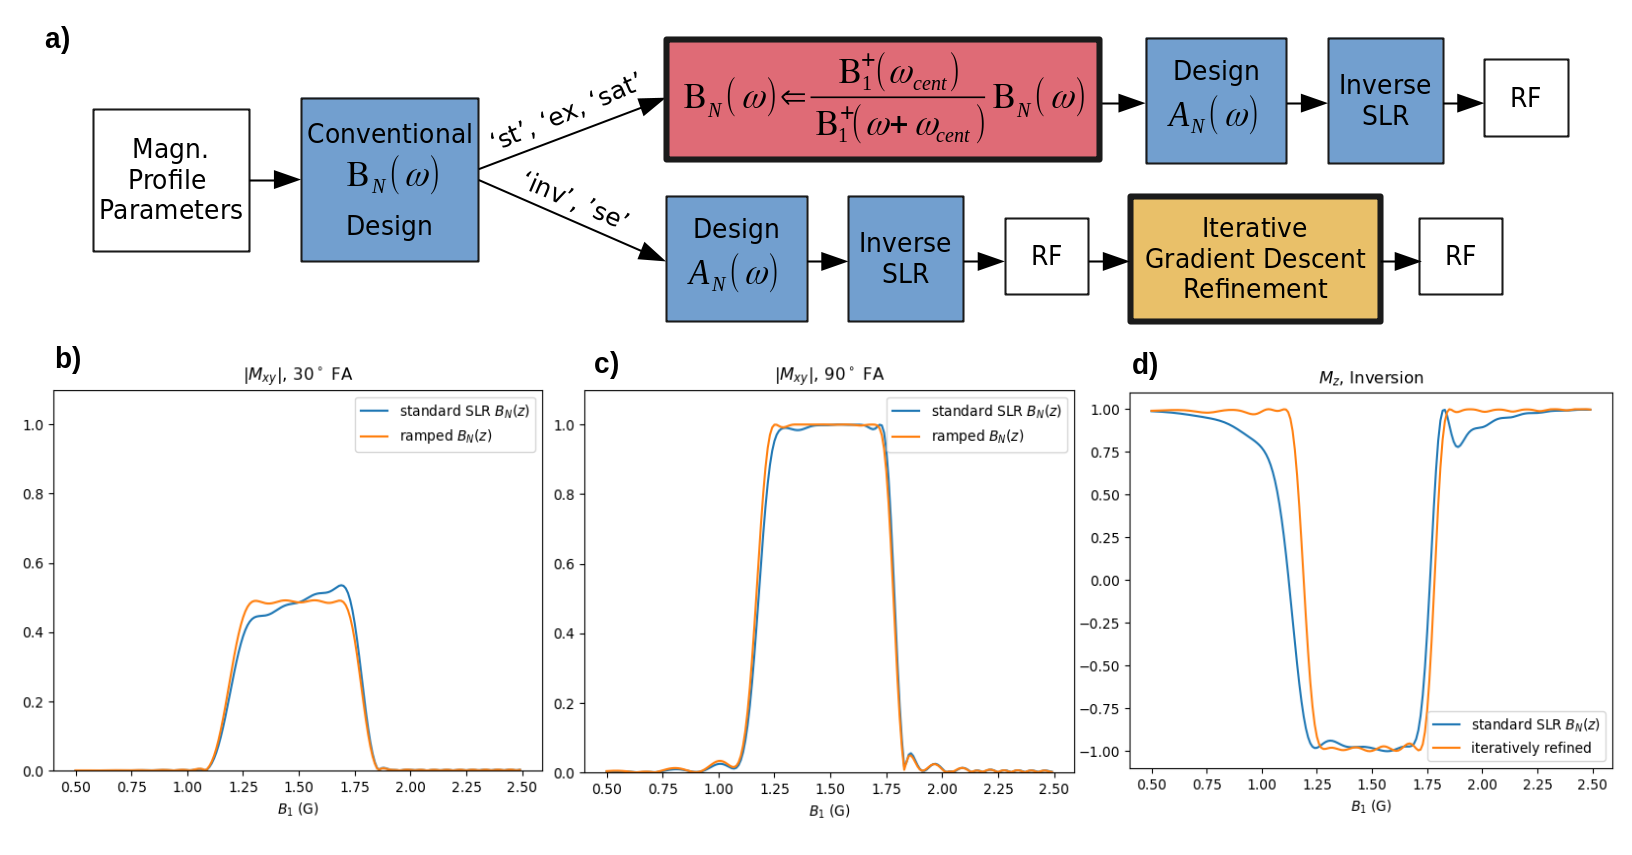
\includegraphics[width=1\textwidth]{figures/beta_filt_flowchart.png}
\caption{a) SLR design algorithm to compensate for a sloped excitation profile across $B_1^+$. In the case of small-tip (`st') or 90° (`ex', `sat') excitation, a
pointwise scaling of the $B_N (\omega)$ profile is sufficient. 
For an inversion (`inv') or refocusing (`se') pulse, iterative refinement is required. 
b) Uncorrected and corrected 30°, PBC = 1.4 G, PBW = 0.6 G, $T_{ex}B=8$ excitation.
c) Uncorrected and corrected 90° excitation. 
d) Uncorrected and corrected inversion profile after
autodifferentiated gradient descent optimization of the pulse with respect to its magnetization profile, Iterative refinement corrected the highly distorted transition bands of the profile.}
\label{fig:ramp}
\end{figure}

%%%%%% FIGURE 4 %%%%%%%
\begin{figure}[h]
\centering
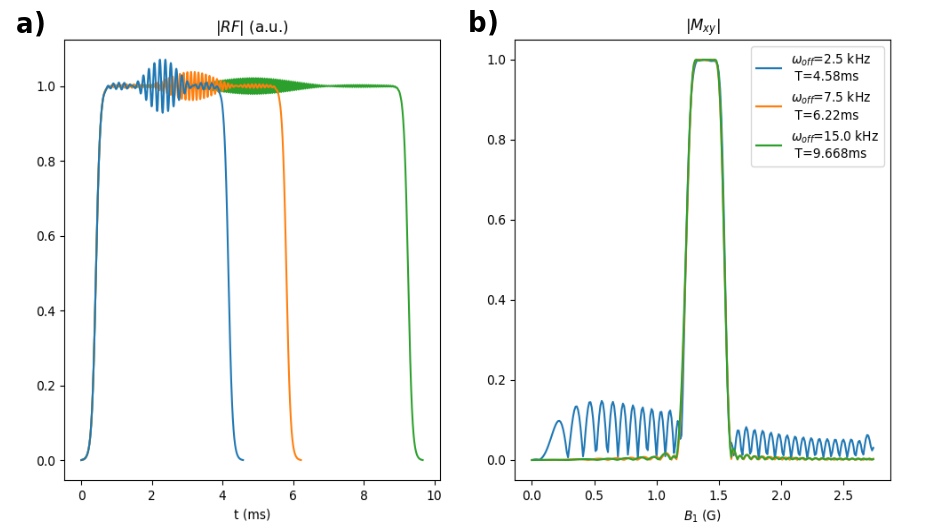
\includegraphics[width=1\textwidth]{figures/bs_offset_comparison_processed.png}
\caption{Comparison of magnetization profiles produces by BSSE pulses with varying $\omega_{off}$. 
a) Increasing $\omega_{off}$ increases minimum pulse duration, 
due to the reduced bandwidth produced by the smaller Bloch-Siegert shift across $B_1^+$. 
b) Larger offsets can help to reduce out-of band excitation. 
A pulse with $\omega_{off}$ = 2.5 kHz produces a substantial amount of out-of-band excitation, 
which is reduced to within design specifications when $\omega_{off} \rightarrow$ 7.5 kHz. 
Continuing to increase $\omega_{off}$ to 15.0 kHz did not further improve the profile.}
\label{fig:bsse_offres_comp}
\end{figure}


%%%%%% FIGURE 5 %%%%%%%
\begin{figure}[h]
\centering
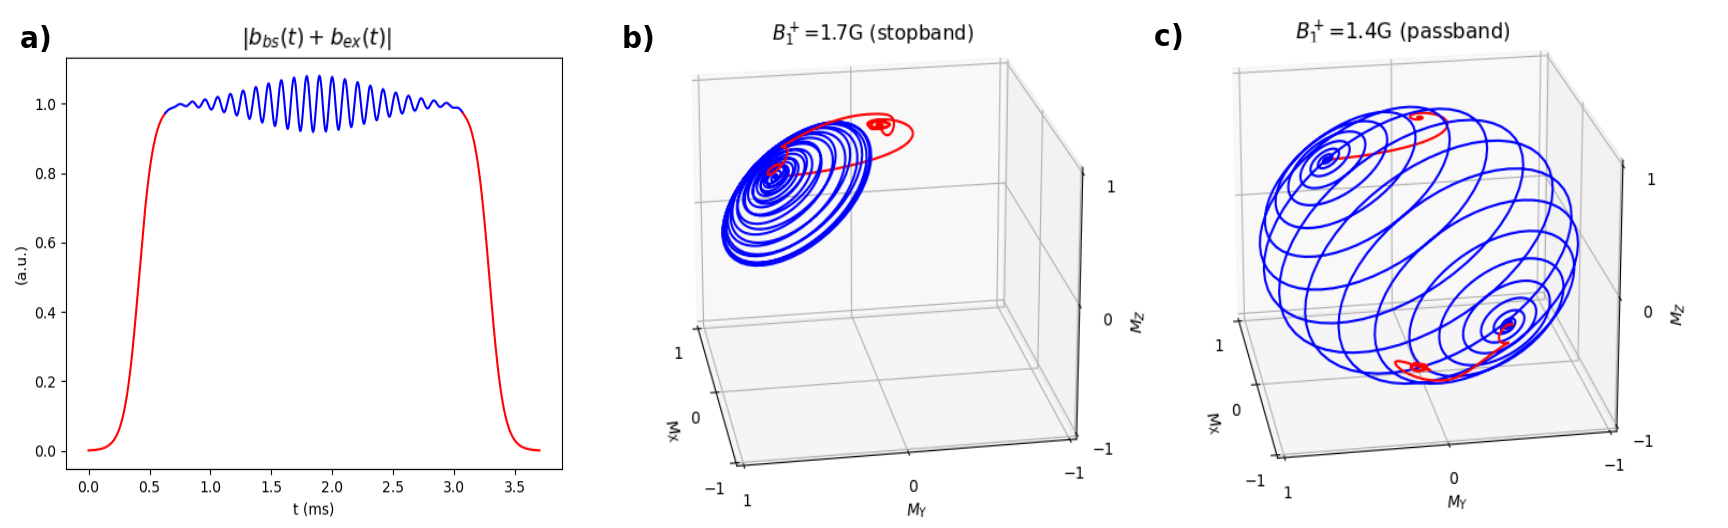
\includegraphics[width=1.1\textwidth]{figures/trajectory_figure.png}
\caption{a) Magnitude of a $T = 3.7$ ms BSSE inversion pulse. 
The pulse is colored red during the adiabatic frequency sweeps when $\bext = 0$, and blue during the constant portion of $\bbst$ when $\bext \neq 0$. 
b) Motion of the net magnetization vector in the $\omega_{off}$ rotating frame for a stopband isochromat. 
The simulation timestep was 4 $\mu$s. At the end of the pulse, magnetization is essentially unperturbed.
c) Motion of the net magnetization vector in the $\omega_{off}$ rotating frame for a passband isochromat. 
At the end of the pulse, magnetization is successfully inverted.}
\label{fig:motion}
\end{figure}

%%%%%% FIGURE 6 %%%%%%%
\begin{figure}[h]
\centering
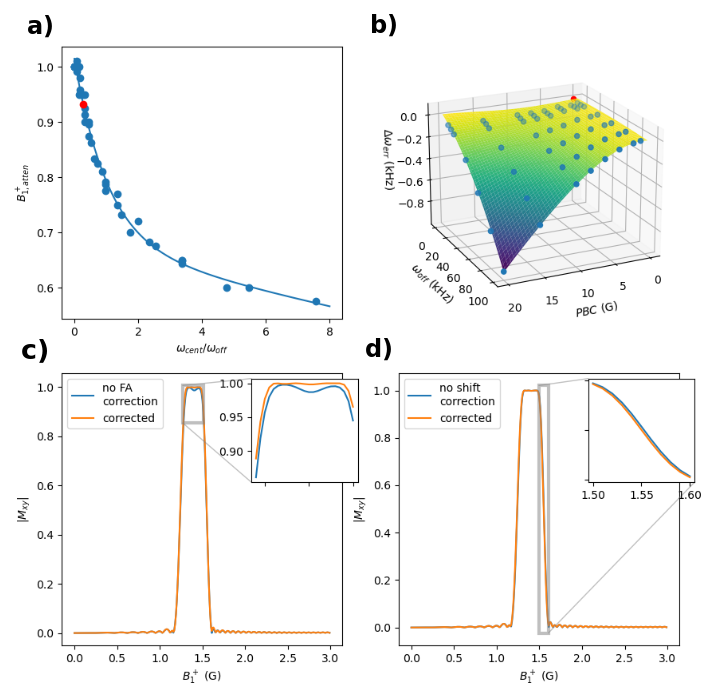
\includegraphics[width=1.\textwidth]{figures/correction_fact_processed.png}
\caption{a) Flip angle attenuation factor versus $ \omega_{cent}/\omega_{off}$.
Data points are empirical correction factors found through simulation, 
with an exponential fit to the data shown as a continuous line. 
The red dot indicates the parameters of the pulse simulated in (c) and (d). 
b) $\Delta \omega_{err}$ correction versus $\omega_{off}$ and $B_1^+$ PBC.  
Data points indicate empirical correction factors found through simulation, 
with a 2D polynomial fit to the data shown as a continuous surface. 
c) Excited slice profile of a PBC =1.4 Gauss, PBW = 0.3 Gauss, 
$90^\circ$, $\omega_{off}$=7.5 kHz pulse with and without the empirical FA correction. 
Applying the correction improves the effective flip angle of the pulse. 
d) Profile from same pulse as (c), 
with and without the empirical $\Delta \omega_{err}$ correction. 
The difference is minimal at this $B_1^+$ and $\omega_{off}$.
}
\label{fig:corrs}
\end{figure}

%%%%%% FIGURE 7 %%%%%%%
\begin{figure}[h]
\centering
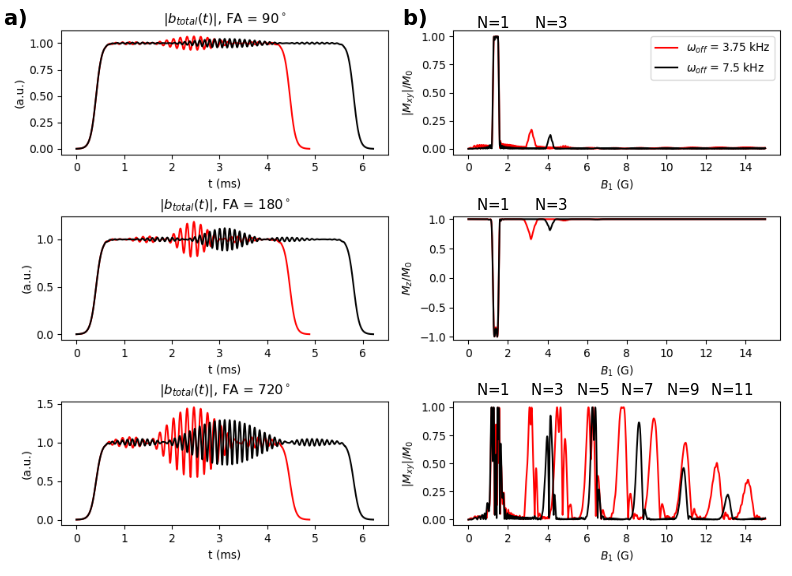
\includegraphics[width=1.1\textwidth]{figures/multiphoton_processed.png}
\caption{a) Magnitudes of $90^\circ$, $180^\circ$, and $720^\circ$ BSSE pulses with $\omega_{off}$ = 7.5 kHz (black) and $\omega_{off}$= 15.0 kHz (red). 
b) The corresponding simulated magnetization profiles. 
Multiphoton resonances are visible at the locations in $B_1^+$ predicted by Equation $\ref{eq:mp_b1}$. 
Increasing $\omega_{off}$ shifts resonances $N \geq 3$ upward in $B_1^+$.}
\label{fig:multiphoton}
\end{figure}

%% Comment: add legend


%%%%%% FIGURE 8 %%%%%%%
\begin{figure}[h]
\centering
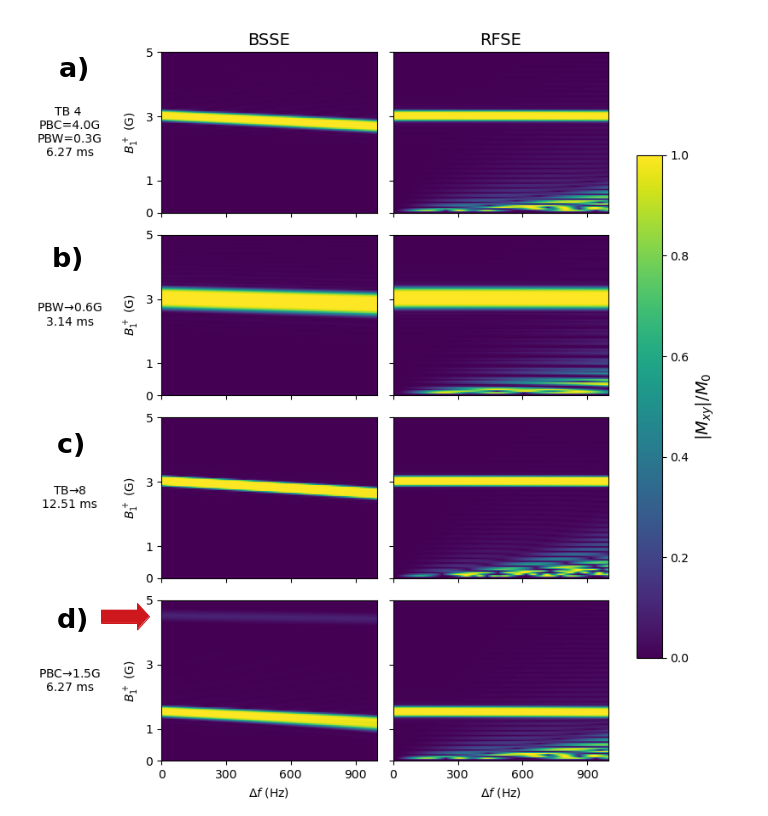
\includegraphics[width=0.8\textwidth]{figures/offres_processed.png}
\caption{Simulations of BSSE and RFSE pulse off-resonance sensitivity. 
a) Simulation of the ``base'' 6.27ms BSSE and RFSE pulses with TB=4, PBC=4.0G, PBW=0.3G, FA=90$^\circ$. 
$\omega_{off}$ was set to  16.37 kHz to match the RFSE pulse duration. 
b) Same as base pulse but with PBW set to 0.6 G. 
$\omega_{off}$ was set to 9.48 kHz to match durations. 
c) Same as base but with TB set to 8. 
$\omega_{off}$ was set to 19.25 kHz to match durations. 
d) Same as base but with PBC set to 1.5 G. 
$\omega_{off}$ was set to 8.17 kHz to match durations.
In all cases, the BSSE magnetization profiles show a bulk shift in the magnetization profile with increasing off-resonance. 
The red arrow in d) shows the location of an $N=3$ multiphoton resonance. 
This multiphoton resonance also experiences a bulk shift down in $B_1^+$ with increasing off-resonance. 
The RFSE profiles show no bulk shift, but have substantial unintended excitation at low $B_1^+$.}
\label{fig:offres}
\end{figure}

%%%%%% FIGURE 9 %%%%%%%
\begin{figure}[h]
\centering
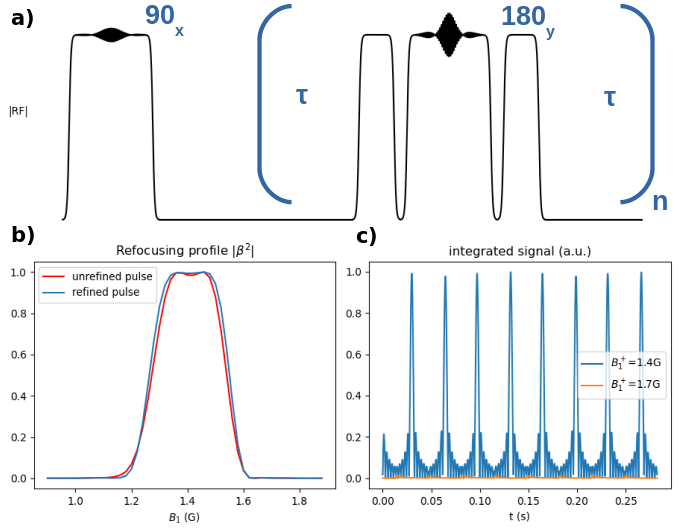
\includegraphics[width=1\textwidth]{figures/cpmg_oneb1_refined_processed.png}
\caption{BSSE Multi-echo CPMG pulse sequence. 
a) Pulse sequence diagram. A 90$^\circ$ excitation pulse was followed by a train of 180$^\circ$ pulses. 
The frequency-swept Fermi RF pulses of \S 2.1 were used in place of refocusing gradients. 
b) $|\beta^2|$ refocusing efficiency profile for the refocusing pulse. 
Refocusing was selective and nearly complete across the passband. 
The gradient descent-refined 180$^\circ$ pulse had a more selective and wider profile, 
although the unrefined pulse also performs well given the narrow PBW. 
c) Signal timecourse in the passband and stopband. 
Regularly spaced echos of uniform amplitude were produced in the passband.}
\label{fig:cpmg}
\end{figure}



%%%%%% FIGURE 10 %%%%%%%
\begin{figure}[h]
\centering
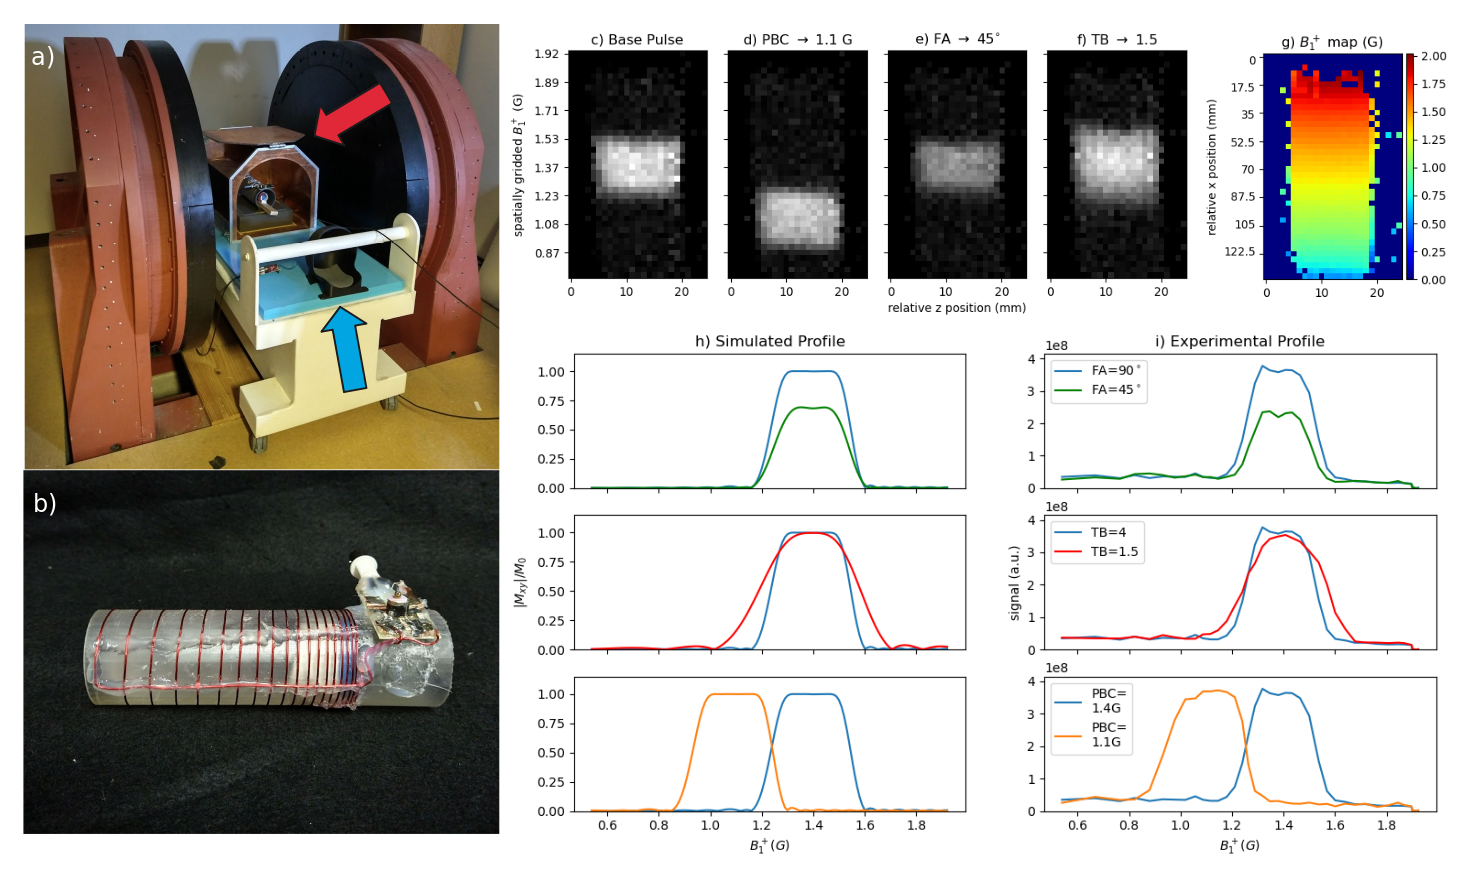
\includegraphics[width=1.1\textwidth]{figures/experimental_2D_processed_Rev2.png}
\caption{Simulated and experimental signal profiles. 
a) 45$^\circ$ (green) versus 90$^\circ$ (blue) excitations. The 90$^\circ$ excitation produces higher signal intensity.
b) TB = 1.5 (red) and TB = 4 (blue) excitations. The TB = 1.5 excitation has a broader transition width.
c) PBC = 1.1 G (orange) and PBC = 1.4 G (blue) excitations. The PBC = 1.1 G excitation is shifted downward by the desired amount.
}
\label{fig:exp}
\end{figure}

\renewcommand{\figurename}{Supporting Information Figure}
\renewcommand\thefigure{S\arabic{figure}}
\setcounter{figure}{0}

% %%%%%% FIGURE S1 %%%%%%%
% \begin{figure}[h]
% \centering
% 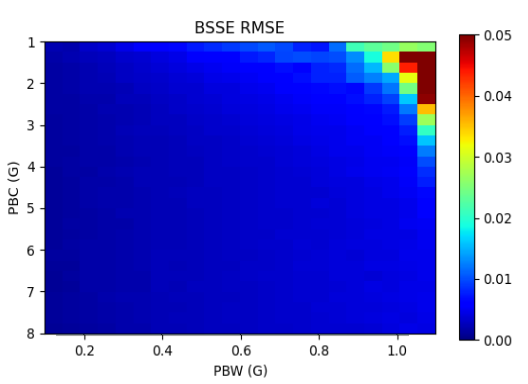
\includegraphics[width=0.8\textwidth]{figures/bsse_rmse.png}
% \caption{\textcolor{red}{WAG: Needs to be discussed in Results.} 
% BSSE magnetization profile RMSE for a pulse with $\omega_{off}$=7.5kHz, TB=4, FA=$90^\circ$. Across a broad range of PBW and PBC, the BSSE pulse has extremely low RMSE. However, in the regime in which the PBW becomes large relative to the PBC (top right), error sharply increases. This is primarily due to the nonlinearity of the Bloch-Siegert shift at low $B_1^+$}
% \label{fig:bsse_rmse}
% \end{figure}

%%%%%% FIGURE S1 %%%%%%%
\begin{figure}[h]
\centering
\includegraphics[width=1.1\textwidth]{figures/magmotion_appendix.gif}
\caption{\textcolor{blue}{JBM: gif does not render in pdf. Figure attached in 'figures' folder: 'magmotion appendix.gif'} a) Magnitude of a $T = 3.7$ ms BSSE inversion pulse. 
The red trace is 10 $\mu$s long. 
b) Stopband magnetization trajectory in the $\omega_{off}$ rotating frame. 
The Simulation timestep was 4 $\mu$s.
c) Passband magnetization trajectory in the $\omega_{off}$ rotating frame.}
\label{fig:magmotion_animated}
\end{figure}
